\documentclass{sig-alternate}

\begin{document}
%
% --- Author Metadata here ---
%\conferenceinfo{WOODSTOCK}{'97 El Paso, Texas USA}
%\CopyrightYear{2007} % Allows default copyright year (20XX) to be over-ridden - IF NEED BE.
%\crdata{0-12345-67-8/90/01}  % Allows default copyright data (0-89791-88-6/97/05) to be over-ridden - IF NEED BE.
% --- End of Author Metadata ---

\title{ContextAmber: Context-oriented Programming in Amber~Smalltalk}

\numberofauthors{1} %  in this sample file, there are a *total*
\author{
\alignauthor
Matthias Springer\\
       \affaddr{Hasso Plattner Institute, Software Architecture Group}\\
       \email{matthias.springer@student.hpi.uni-potsdam.de}
}

\date{\today}
% Just remember to make sure that the TOTAL number of authors
% is the number that will appear on the first page PLUS the
% number that will appear in the \additionalauthors section.

\maketitle
\begin{abstract}
Amber Smalltalk is an implementation of the Smalltalk programming language in JavaScript. It consists of a Smalltalk-to-JavaScript compiler, an IDE running in a web browser, and an optional NodeJS-based backend for saving changed source code files to the disk. Context-oriented programming is a tool for modularizing cross-cutting concerns in object-oriented programming languages. We present ContextAmber, a framework for context-oriented programming that is integrated in Amber Smalltalk and itself written in Amber Smalltalk.

ContextAmber hooks into the Smalltalk compiler, which is also written in Amber Smalltalk, and adds a decorator method that checks the current layer composition and executes partial methods. It also optimizes partial method execution by inlining them into a single method if the layer composition does not change for some time.

As a running example, we show how to implement a simple method profiler that evaluates method calls following a certain pattern. The profiler measures the running time of Smalltalk methods and analyzes method parameters. By doing so, we can gather valuable information for program optimization.
\end{abstract}

% A category with the (minimum) three required fields
%\category{H.4}{Information Systems Applications}{Miscellaneous}
%A category including the fourth, optional field follows...
%\category{D.2.8}{Software Engineering}{Metrics}[complexity measures, performance measures]

%\terms{Theory}

%\keywords{ACM proceedings, \LaTeX, text tagging}

\section{INTRODUCTION}
Modern web applications depend highly on the usage of JavaScript. Since the JavaScript programming language itself is pretty limited and hard to use, web developers soon started to write frameworks and libraries for JavaScript (e.g., jQuery or AngularJS). These libraries fulfill different purposes, but they all focus on making it easier to write JavaScript applications in JavaScript. Amber Smalltalk uses a different approach: it allows the programmer to write his code in the more structured and class-oriented programming language Smalltalk.

In this work, we present ContextAmber, a framework for context-oriented programming, that allows the programmer to modularize heterogeneous crosscutting concerns. A concern is crosscutting, if parts of its implementation are scattered across different modules of the program. A crosscutting concern is heterogeneous if its implementation requires different behavior for every module where it leaks through. The most important concepts of context-oriented programming are partial method definitions, layers, and dynamic layer activation.

\paragraph{Partial Method Definitons}
In context-oriented programming, the behavior of base methods is extended by partial methods. A partial method overrides a certain base method and, therefore, replaces its original behavior. It can still \emph{proceed} to the original base method at any point. Partial methods are similar to \emph{around advice} in aspect-oriented programming.

\paragraph{Layers}
A layer encapsulates a set of partial methods that belong together conceptually. Layers can be instantiated and have instance methods like classes.

\paragraph{Dynamic Layer Activation}
Layers can be activated and deactivated, resulting in partial methods being called instead of their base methods or not. Layer activation is dynamic in a sense that we can turn layers on and off at runtime with designated methods calls or with expressions that are new to the programming language's syntax.

\section{RELATED WORK}
A variety of implementations for context-oriented programming with different features exists. JCop is an implementation for Java and supports declarative layer composition: instead of activating or deactivating layers explicitly, we specify a boolean expression which activates a layer automatically if it holds true. This fits nicely with the idea that the \emph{context} is anything that can be calcuated computationally, and that behavior changes automatically once the context changes.

ContextJS is an implementation for JavaScript and integrated into the Lively Kernel. It supports layer activation and deactivation based on the composition of morphs, in addition to global layer activation, scoped layer activation, and object-wise layer activation.

Aspect-oriented programming is a way to modularize homogeneous crosscutting concerns. Partial methods are called pieces of \emph{advice} and modularized in \emph{aspects}. A special \emph{pointcut} notation defines with which base method a piece of advice will be executed. Typically, one piece of advice will be applied to multiple base methods, which is why aspect-oriented programming is suitable for homogeneous crosscutting concerns. Advice code can not only replace a base method (\emph{around} advice), but also be executed before or after the base method was executed. Aspect-oriented programming is a superset of context-oriented programming with the only limitation that most implementations for aspect-oriented programming are static (i.e., the programmer has to specify at compile time where pieces of advice should be applied).

Context-oriented programming is less powerful than aspect-oriented programming, making it easier to reason about layers and layer composition.

\section{AMBER'S OBJECT MODEL}
Amber Smalltalk implements an object model that is similar to the Smalltalk-80 object model. Amber Smalltalk is purely object-oriented and every Smalltalk object is a JavaScript object at the same time; however, not every JavaScript object is a Smalltalk object in a sense that arbitrary JavaScript objects do not have Smalltalk instance variables or Smalltalk instance methods\footnote{See Section~? for details on Smalltalk-JavaScript integration.}. Smalltalk instance variables are stored as JavaScript properties with an \texttt{@} prefix. An object's instance methods are stored in its prototype object as properties but never in the object itself. They always begin with an \texttt{\_} prefix.

\begin{figure}[h]
\centering
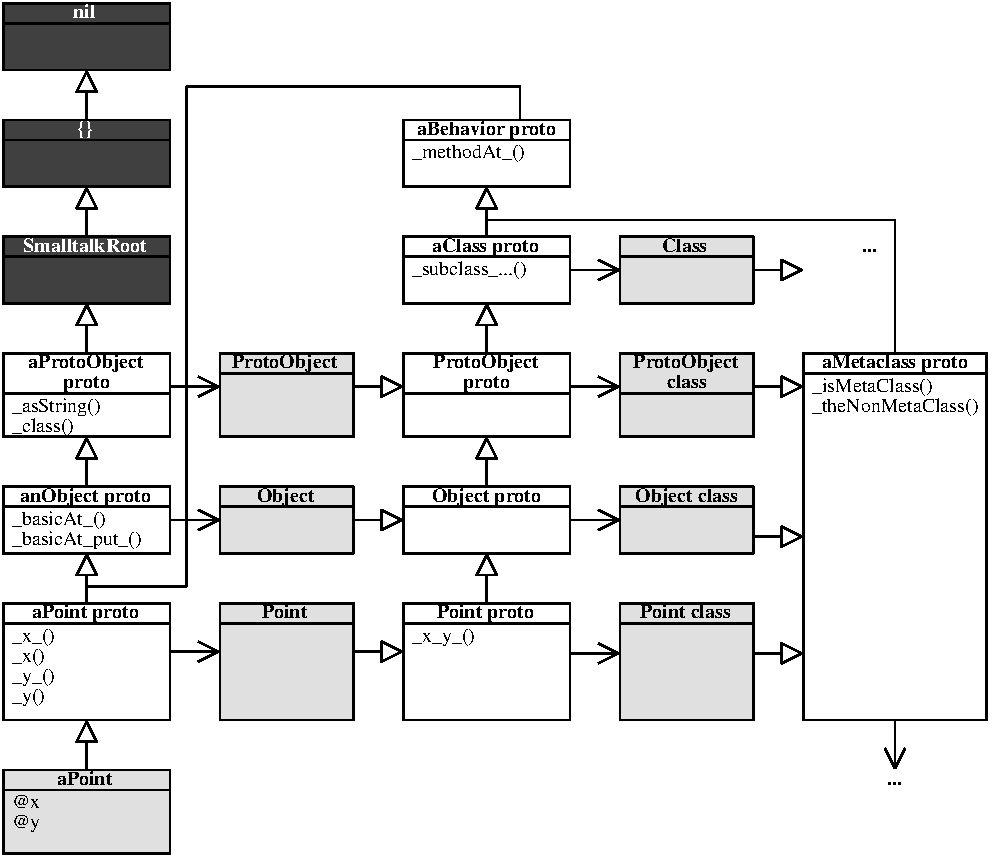
\includegraphics[width=0.49\textwidth]{amber_class_model.pdf}
\label{fig:amber_obj}
\caption{Part of Amber's object model as seen from the JavaScript side. Inheritance arrows designate prototype chains. An association arrow between object \texttt{a} and object \texttt{b} means that \texttt{a.klass = b}.}
\end{figure}

Figure~\ref{fig:amber_obj} shows a part of Amber Smalltalk's object model. As an example, consider the object \texttt{aPoint} which is an instance of the Smalltalk class \texttt{Point} and represents a 2D point with an x and a y coordinate. The corresponding instance variables are stored in \texttt{aPoint} directly. Its instance methods are stored in \texttt{aPoint proto}. All point instances have this object as a prototype. If we follow the prototype chain, we will get all of  \texttt{Point}'s super classes, and eventually reach an empty JavaScript object and, finally, \texttt{nil}. An object's class reference is stored in the JavaScript property \texttt{klass}. \texttt{ProtoObject proto}'s prototype is \texttt{aClass proto}, which is why every Smalltalk class is also \texttt{anObject}. Note, that \texttt{ProtoObject proto} corresponds to \texttt{ProtoObject}'s class side in Smalltalk, whereas \texttt{aClass proto} corresponds to \texttt{Class}' instance side in Smalltalk.


\section{COMPILATION PROCESS}
Amber Smalltalk compiles Smalltalk to JavaScript when a method is saved or a statement is executed in the workspace. In either case, the method \texttt{Compiler>>compile:} is called with the Smalltalk source code as an argument. It returns the JavaScript source code. The following list gives an overview of the compilation process.

\begin{enumerate}
    \item Smalltalk source code parsing. The parser is generated from a \emph{parsing expression grammar} using the PEG.js parser generator. The parser outputs an abstract syntax tree (AST).
    \item Semantic analysis. Examples are checking if an identifier is defined (i.e., if a variable/class/argument/JavaScript variable with that name exists), or checking for variable shadowing which is not allowed in Smalltalk.
    \item AST to Intermediate Representation (IR) conversion. This step involves inlining message sends for \texttt{ifTrue:}, \texttt{ifFalse:}, \texttt{ifTrue:ifFalse:}, and \texttt{ifNil:ifNotNil:}.
    \item JavaScript code generation. JavaScript code is generated while traversing the IR tree.
\end{enumerate}

\section{OUR IMPLEMENTATION}
In this section, we describe the main ideas of our implementation. We first present an unoptimized implementation and will then show how to speed up our implementation.

\subsection{DATA STRUCTURE}
In context-oriented programming, we modularize partial methods in layers. Every partial method belongs to exactly one base method in a specific class. In ContextAmber, a layer is an instance of a subclass of the class \texttt{Layer}. We consider several alternatives for associating partial methods with base classes.

\paragraph{Class name prefix}
We create a class for every layer. The names of partial methods are a combination of the base class name and the base method name. Consider, for example, that we want to define a layer \texttt{RotationLayer} for the base method \texttt{Point>>x:}. The name of the partial method would be \texttt{RotationLayer>>Point\$x:}. The dollar sign has no meaning in Amber Smalltalk but is also not allowed in identifiers. Implementing this approach requires changing the grammar, such that the dollar sign is allowed in method names, and adding a check to the semantic analyzer that ensures that method names with a single dollar sign are allowed only in methods defined in a layer.

\paragraph{Method protocols}
Instead of prefixing partial method names, the partial method's protocol is the name of the base class; however, this restricts us in categorizing partial methods in a meaningful way.

\paragraph{Partial classes}
A layer definition consists of multiple classes. For every base class for which a partial method exists, there is a separate class containing all partial methods for that base class. We call these classes partial classes. In addition, there is a central layer class maintaining all layer-specific state and aggregating all partial classes for that layer. We use partial classes in ContextAmber, but other implementations typically use class name prefixes (e.g., JCop and ContextJS).

\subsection{LAYER ACTIVATION}

\paragraph{Global layer activation}
% Was wenn Layer global aktiv aber dann im Scope ausgeschaltet?

\paragraph{Object-wise layer activation}

\paragraph{Scoped layer activation}

\section{PROFILING SMALLTALK METHODS}
Talk about the Smalltalk method profiler.

\section{FUTURE WORK}
Talk about what still needs to be done.

\section{CONCLUSION}

\end{document}
